\documentclass[a4paper,fleqn]{cas-sc}

% -----------------------------------------------------------------------------
% PACKAGE CONFIGURATION ACCORDING TO ELSEVIER CAS-SC TEMPLATE
% -----------------------------------------------------------------------------
\usepackage[utf8]{inputenc}
\usepackage[T1,T5]{fontenc}
\usepackage[english]{babel}

\usepackage{subcaption}
\usepackage{tabularx}
\usepackage{longtable}
\usepackage{algorithm}
\usepackage{algpseudocode}

% Theorem environments
\newtheorem{theorem}{Theorem}
\newtheorem{lemma}[theorem]{Lemma}
\newtheorem{definition}{Definition}
\newtheorem{proposition}[theorem]{Proposition}

% Algorithm caption name
\floatname{algorithm}{Algorithm}

\begin{document}
\let\WriteBookmarks\relax
\renewcommand{\topfraction}{.9}
\renewcommand{\bottomfraction}{.8}
\renewcommand{\textfraction}{.1}
\renewcommand{\floatpagefraction}{.75}

% Short title and short authors for running header
\shorttitle{Empirical Study of SAT Encodings for N-Queens}
\shortauthors{Tran Nhat Hung}

% Main article title
\title [mode = title]{AN EMPIRICAL STUDY ON SAT ENCODING TECHNIQUES AND MULTI-PARADIGM COMPARISON (SAT, CP, MIP) FOR THE N-QUEENS PROBLEM}

% Author information
\author{Tran Nhat Hung}
\ead{24021507@vnu.edu.vn}

\address{Faculty of Information Technology, VNU University of Engineering and Technology, 144 Xuan Thuy, Cau Giay, Hanoi, Vietnam}

\nonumnote{Course Project Report 1 -- Course: Modern Topics in Computer Science (Course ID: INT3011E 3). Instructor: Dr. To Van Khanh. Student: Tran Nhat Hung -- Student ID: 24021507.}

% Abstract
\begin{abstract}
The $N$-Queens problem is a classic benchmark in combinatorial optimization, automated reasoning, and formal verification. When the chessboard scale expands to large dimensions ($N \ge 500$, corresponding to millions of Boolean variables), the exponential explosion of the search space requires modeling methods and exact solvers to deliver exceptional performance. In this study, we implement two deep empirical research axes: (1) Investigating and benchmarking five At-Most-One (AMO) constraint encoding techniques into SAT, including Binomial (Pairwise), Binary (Bitwise), Sequential Counter, Commander Variable ($g=3$), and 2-Product on the Glucose4 solver; (2) Extending a cross-paradigm benchmark between SAT Solving and two baseline exact computing paradigms: Constraint Programming (CP: Google OR-Tools CP-SAT, IBM ILOG CPLEX CP Optimizer) and 0-1 Mixed Integer Programming (MIP: Gurobi Optimizer, IBM ILOG CPLEX MIP) across a synchronized benchmark suite of 15 board sizes from $N = 4$ to $N = 1000$. Experimental results demonstrate that the Binomial encoding explodes with $O(N^4)$ clauses, causing Out-Of-Memory (OOM) failures at $N \ge 512$. Conversely, although the Sequential Counter technique preserves Generalized Arc Consistency (GAC), it suffers from the \textit{Sequential Counter Paradox}, where millions of auxiliary variables dilute the CDCL solver's VSIDS branching heuristic, leading to timeouts. The Commander Variable and Binary encodings achieve an ideal balance, successfully solving all 15 benchmark instances up to $N = 1000$ (with Commander solving $N=1000$ in only $20.10$ seconds). In the cross-paradigm comparison, IBM CPLEX CP Optimizer exhibits absolute dominance ($0.250$ seconds for $N = 1000$) due to compact $N$-integer-variable modeling and R{\'e}gin's filtering propagation for the global AllDifferent constraint. Notably, PySAT Glucose4 Commander completes $N = 1000$ in $18.92$ seconds, outperforming both major commercial solvers, Gurobi MIP (Timeout) and OR-Tools CP-SAT (Timeout). All source code, empirical datasets, and measurement results are publicly available at GitHub: \url{https://github.com/NhHung07/N_Queens.git}.
\end{abstract}

% Keywords
\begin{keywords}
N-Queens \sep SAT Solving \sep At-Most-One Encoding \sep Constraint Programming \sep Mixed Integer Programming \sep CDCL \sep PySAT
\end{keywords}

\maketitle

% =============================================================================
% SECTION 1: INTRODUCTION
% =============================================================================
\section{Introduction}
\label{sec:intro}

\subsection{Problem Definition}
\label{subsec:problem_def}
The $N$-Queens problem is a classic benchmark in artificial intelligence, combinatorial optimization, and automated reasoning \cite{letavec2002nqueens}. Originally formulated by chess player Max Bezzel in 1848 for an $8 \times 8$ chessboard \cite{bezzel1848} and generalized by Franz Nauck to an $N \times N$ board in 1850 \cite{nauck1850}, the objective is to place $N$ non-attacking queens on an $N \times N$ chessboard such that no two queens can threaten each other.

\begin{figure}[pos=htbp]
    \centering
    \begin{subfigure}[b]{0.45\textwidth}
        \centering
        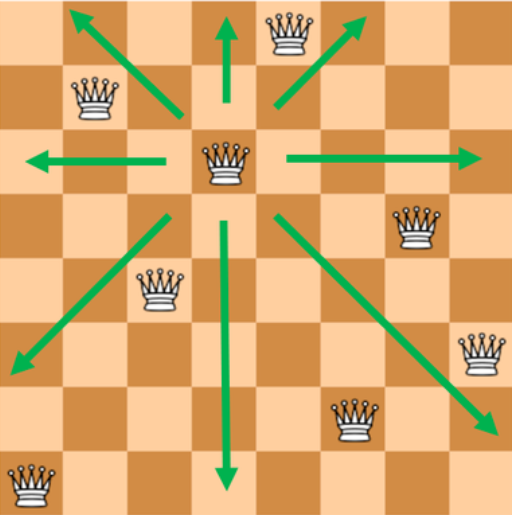
\includegraphics[width=0.88\linewidth]{figures/nqueens_valid.png}
        \caption{Valid solution configuration}
        \label{fig:valid_queen}
    \end{subfigure}
    \hfill
    \begin{subfigure}[b]{0.45\textwidth}
        \centering
        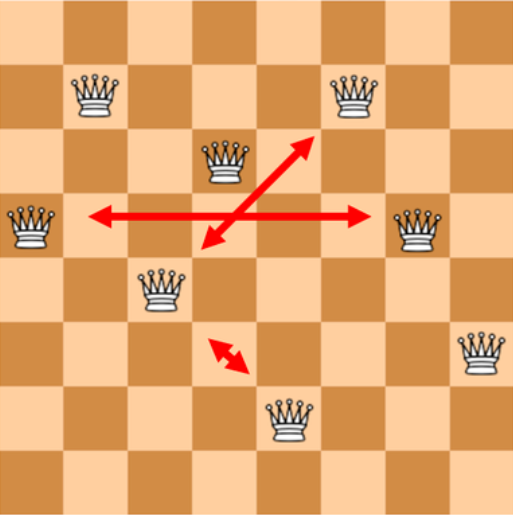
\includegraphics[width=0.88\linewidth]{figures/nqueens_invalid.png}
        \caption{Constraint violation configuration}
        \label{fig:invalid_queen}
    \end{subfigure}
    \caption{Visual illustration of a valid solution configuration versus a conflicting configuration on the $N$-Queens chessboard.}
    \label{fig:nqueens_illustration}
\end{figure}

Figure~\ref{fig:nqueens_illustration} illustrates the visual distinction between a valid configuration and a conflicting configuration:
\begin{itemize}
    \item \textbf{Figure~\ref{fig:valid_queen} (Valid solution):} Every queen occupies an independent position, sharing no common row, column, or diagonal with any other queen.
    \item \textbf{Figure~\ref{fig:invalid_queen} (Conflicting configuration):} There exist multiple queens situated on the same row, column, or diagonal, directly attacking each other.
\end{itemize}

\subsection{Rules of the N-Queens Problem}
\label{subsec:rules}
Under standard international chess rules, the queen is the most versatile and powerful piece on the board: it can move an arbitrary number of unobstructed squares horizontally (along rows), vertically (along columns), and diagonally (along both main diagonals and anti-diagonals). Consequently, placing $N$ queens on an $N \times N$ chessboard must simultaneously satisfy four prerequisite conditions:
\begin{enumerate}
    \item No two queens share the same row (Row constraint).
    \item No two queens share the same column (Column constraint).
    \item No two queens share the same main diagonal (Main diagonal constraint).
    \item No two queens share the same anti-diagonal (Anti-diagonal constraint).
\end{enumerate}

Since the chessboard contains exactly $N$ rows and $N$ columns, and exactly $N$ queens must be placed, by Dirichlet's pigeonhole principle, each row and each column must contain \textbf{exactly one queen} (Exactly-One). Meanwhile, each diagonal can contain \textbf{at most one queen} (At-Most-One).

\subsection{Practical Applications of the Problem}
\label{subsec:apps}
Far beyond a recreational mathematical puzzle, mathematical models derived from the $N$-Queens problem are intimately connected to and widely applied across numerous modern engineering domains \cite{sosic1994polynomial,erbas1992queens}:
\begin{itemize}
    \item \textbf{VLSI (Very Large Scale Integration) Circuit Design and Verification:} Optimizing routing paths and non-conflicting component placement across semiconductor integrated circuit layers.
    \item \textbf{Scheduling and Computational Resource Management:} Register allocation in optimizing compilers and deadlock prevention in multithreaded process scheduling.
    \item \textbf{Telecommunications and Optical Routing:} Wavelength assignment in wavelength-division multiplexing (WDM) optical networks ensuring parallel channels do not produce cross-talk interference.
    \item \textbf{Aviation and Air Traffic Management:} Runway slot allocation and landing flight scheduling at major international hubs.
    \item \textbf{Permutation Problems and Traveling Salesperson (TSP):} Formulating combinatorial permutation constraints in logistics routing optimization \cite{hoffman2013traveling}.
\end{itemize}

\subsection{Traditional Solving Approaches}
\label{subsec:traditional}
Early algorithmic approaches for solving the $N$-Queens problem relied primarily on exhaustive tree search combined with pruning techniques:

\paragraph{1. Backtracking Algorithm:}
The algorithm traverses sequentially through each row (or column), places a queen at the first available conflict-free square, and recursively proceeds to the next row \cite{golomb1965backtrack}. If a dead-end state is encountered where no safe square remains, the algorithm backtracks to the previous row to try alternative positions. The procedure is formally detailed in Algorithm~\ref{alg:backtrack}.

\begin{algorithm}[htbp]
\caption{Solving the $N$-Queens Problem using Backtracking}
\label{alg:backtrack}
\begin{algorithmic}[1]
\Function{solveNQueens}{$N$}
    \State Initialize array $\text{board}$ of size $N$ with elements set to $-1$
    \State \Call{solveNQueensUtil}{$\text{board}, 0, N$}
\EndFunction
\Statex
\Function{solveNQueensUtil}{$\text{board}, \text{row}, N$}
    \If{$\text{row} = N$}
        \State Print solution configuration $\text{printBoard}(\text{board})$
        \State \Return $\mathbf{True}$
    \EndIf
    \For{$\text{col} = 0$ \textbf{to} $N-1$}
        \If{\Call{isSafe}{$\text{board}, \text{row}, \text{col}, N$}}
            \State $\text{board}[\text{row}] \gets \text{col}$ \Comment{Place queen at safe position}
            \If{\Call{solveNQueensUtil}{$\text{board}, \text{row} + 1, N$}}
                \State \Return $\mathbf{True}$
            \EndIf
            \State $\text{board}[\text{row}] \gets -1$ \Comment{Backtrack: Remove queen}
        \EndIf
    \EndFor
    \State \Return $\mathbf{False}$
\EndFunction
\Statex
\Function{isSafe}{$\text{board}, \text{row}, \text{col}, N$}
    \For{$i = 0$ \textbf{to} $\text{row}-1$}
        \If{$\text{board}[i] = \text{col}$} \Return $\mathbf{False}$ \Comment{Column conflict}
        \EndIf
        \If{$\text{board}[i] - i = \text{col} - \text{row}$} \Return $\mathbf{False}$ \Comment{Main diagonal conflict}
        \EndIf
        \If{$\text{board}[i] + i = \text{col} + \text{row}$} \Return $\mathbf{False}$ \Comment{Anti-diagonal conflict}
        \EndIf
    \EndFor
    \State \Return $\mathbf{True}$
\EndFunction
\end{algorithmic}
\end{algorithm}

\paragraph{2. Branch and Bound Algorithm:}
To overcome the $O(N)$ safety verification overhead in the $\Call{isSafe}{}$ routine of classic backtracking, the Branch and Bound technique introduces three $O(1)$ state lookup tables: $\text{rowLookup}$ of size $N$, $\text{slashLookup}$ of size $2N-1$ for main diagonals, and $\text{backslashLookup}$ of size $2N-1$ for anti-diagonals \cite{bitner1975backtrack}. The algorithm is formally presented in Algorithm~\ref{alg:branch_and_bound}.

\begin{algorithm}[htbp]
\caption{Solving the $N$-Queens Problem using Branch and Bound}
\label{alg:branch_and_bound}
\begin{algorithmic}[1]
\Function{solveNQueensBB}{$N$}
    \State Initialize array $\text{rowLookup}$ of size $N$ with value $\mathbf{False}$
    \State Initialize $\text{slashLookup}$, $\text{backslashLookup}$ of size $2N-1$ with value $\mathbf{False}$
    \State Initialize board matrix $\text{board}[N][N] \gets 0$
    \State $\text{hasSol} \gets \Call{solveBBUtil}{\text{board}, 0, \text{rowLookup}, \text{slashLookup}, \text{backslashLookup}, N}$
    \If{\textbf{not} $\text{hasSol}$}
        \State \textbf{print} "No solution configuration found"
        \State \Return $\mathbf{False}$
    \EndIf
    \State Print solution configuration $\text{printBoard}(\text{board})$
    \State \Return $\mathbf{True}$
\EndFunction
\Statex
\Function{solveBBUtil}{$\text{board}, \text{col}, \text{rowL}, \text{slashL}, \text{bslashL}, N$}
    \If{$\text{col} \ge N$}
        \State \Return $\mathbf{True}$
    \EndIf
    \For{$\text{row} = 0$ \textbf{to} $N-1$}
        \State $s \gets \text{row} + \text{col}$
        \State $bs \gets \text{row} - \text{col} + (N-1)$
        \If{\textbf{not} $(\text{rowL}[\text{row}] \lor \text{slashL}[s] \lor \text{bslashL}[bs])$}
            \State $\text{board}[\text{row}][\text{col}] \gets 1$
            \State $\text{rowL}[\text{row}] \gets \mathbf{True}$; $\text{slashL}[s] \gets \mathbf{True}$; $\text{bslashL}[bs] \gets \mathbf{True}$
            \If{\Call{solveBBUtil}{$\text{board}, \text{col} + 1, \text{rowL}, \text{slashL}, \text{bslashL}, N$}}
                \State \Return $\mathbf{True}$
            \EndIf
            \State $\text{board}[\text{row}][\text{col}] \gets 0$ \Comment{Backtrack}
            \State $\text{rowL}[\text{row}] \gets \mathbf{False}$; $\text{slashL}[s] \gets \mathbf{False}$; $\text{bslashL}[bs] \gets \mathbf{False}$
        \EndIf
    \EndFor
    \State \Return $\mathbf{False}$
\EndFunction
\end{algorithmic}
\end{algorithm}

Although Branch and Bound substantially accelerates step-level checks, the overall combinatorial search space still scales factorially ($O(N!)$), rendering these traditional tree-traversal algorithms incapable of solving instances beyond $N > 30$.

\subsection{SAT-based Encoding Approach for N-Queens}
\label{subsec:sat_encoding_intro}
To solve the $N$-Queens problem on modern automated reasoning engines, the problem is formulated into Conjunctive Normal Form (CNF). We define an $N \times N$ matrix of Boolean decision variables $B_{i,j}$ ($0 \le i, j < N$):
\begin{equation}
B_{i,j} = \begin{cases}
1, & \text{if a queen is placed at square } (i, j), \\
0, & \text{otherwise.}
\end{cases}
\end{equation}

The problem constraints are decomposed into two fundamental classes of Boolean constraints:
\begin{enumerate}
    \item \textbf{At-Least-One (ALO) constraint:} $\sum_{i=1}^m x_i \ge 1$, simply expressed by exactly one linear disjunctive clause: $(x_1 \lor x_2 \lor \dots \lor x_m)$.
    \item \textbf{At-Most-One (AMO) constraint:} $\sum_{i=1}^m x_i \le 1$.
\end{enumerate}

The requirement that each row and each column contains exactly one queen is formulated as the conjunction of ALO and AMO:
\begin{equation}
\text{Exactly-One}(X) \iff \text{ALO}(X) \land \text{AMO}(X)
\end{equation}

While ALO requires only a single clause, AMO is the central focal point of SAT encoding research. The classical Binomial (Pairwise) encoding explicitly forbids every conflicting pair:
\begin{equation}
\text{AMO}_{\text{Binomial}}(X) = \bigwedge_{j=0}^{m-2} \bigwedge_{k=j+1}^{m-1} (\neg x_j \lor \neg x_k)
\end{equation}
This approach generates $\binom{m}{2} = O(m^2)$ clauses per constraint, which accumulates to a quartic $O(N^4)$ explosion in the total clause count across the entire chessboard, becoming the critical scalability bottleneck.

\subsection{List of Abbreviations}
\label{subsec:abbreviations}
Table~\ref{tab:abbreviations} summarizes the specialized acronyms and abbreviations utilized throughout this paper.

\begin{table}[pos=htbp]
\centering
\caption{List of specialized technical acronyms and abbreviations.}
\label{tab:abbreviations}
\begin{tabular}{ll}
\toprule
\textbf{Acronym} & \textbf{Full Description / Meaning} \\
\midrule
\textbf{ALO} & At-Least-One Constraint \\
\textbf{AMO} & At-Most-One Constraint \\
\textbf{CDCL} & Conflict-Driven Clause Learning \\
\textbf{CNF} & Conjunctive Normal Form \\
\textbf{CP} & Constraint Programming \\
\textbf{CSP} & Constraint Satisfaction Problem \\
\textbf{DPLL} & Davis-Putnam-Logemann-Loveland Algorithm \\
\textbf{GAC} & Generalized Arc Consistency \\
\textbf{ILP} & Integer Linear Programming \\
\textbf{LBD} & Literal Block Distance \\
\textbf{MIP} & Mixed Integer Programming \\
\textbf{OOM} & Out-Of-Memory Error \\
\textbf{SAT} & Boolean Satisfiability Problem \\
\textbf{UNSAT} & Unsatisfiable Instance \\
\textbf{UP} & Unit Propagation \\
\textbf{VSIDS} & Variable State Independent Decaying Sum \\
\textbf{2WL} & Two-Watched Literals Scheme \\
\bottomrule
\end{tabular}
\end{table}

% =============================================================================
% SECTION 2: BACKGROUND
% =============================================================================
\section{Background}
\label{sec:background}

\subsection{Propositional Logic}
\label{subsec:prop_logic}
Propositional logic provides the formal mathematical foundation for studying statements possessing a deterministic truth value: true ($\mathbf{True}$ or $1$) or false ($\mathbf{False}$ or $0$) \cite{simon2020reasoning}. Elementary propositional variables are composed through five standard logical connectives: Negation ($\neg$), Conjunction ($\land$), Disjunction ($\lor$), Implication ($\to$), and Equivalence ($\leftrightarrow$). The comprehensive truth table for these operators is presented in Table~\ref{tab:truth_table}.

\begin{table}[pos=htbp]
\centering
\caption{Truth table of elementary propositional logic operations.}
\label{tab:truth_table}
\begin{tabular}{ccccccc}
\toprule
$A$ & $B$ & $\neg A$ & $A \land B$ & $A \lor B$ & $A \to B$ & $A \leftrightarrow B$ \\
\midrule
$\mathbf{True}$  & $\mathbf{True}$  & $\mathbf{False}$ & $\mathbf{True}$  & $\mathbf{True}$  & $\mathbf{True}$  & $\mathbf{True}$  \\
$\mathbf{True}$  & $\mathbf{False}$ & $\mathbf{False}$ & $\mathbf{False}$ & $\mathbf{True}$  & $\mathbf{False}$ & $\mathbf{False}$ \\
$\mathbf{False}$ & $\mathbf{True}$  & $\mathbf{True}$  & $\mathbf{False}$ & $\mathbf{True}$  & $\mathbf{True}$  & $\mathbf{False}$ \\
$\mathbf{False}$ & $\mathbf{False}$ & $\mathbf{True}$  & $\mathbf{False}$ & $\mathbf{False}$ & $\mathbf{True}$  & $\mathbf{True}$  \\
\bottomrule
\end{tabular}
\end{table}

\subsection{Conjunctive Normal Form (CNF)}
\label{subsec:cnf}
Modern SAT solvers require the input formula to be formulated in Conjunctive Normal Form (CNF):
\begin{itemize}
    \item \textbf{Boolean Variable:} A variable $x \in \{\mathbf{False}, \mathbf{True}\}$.
    \item \textbf{Literal:} A variable or its negation ($x$ or $\neg x$).
    \item \textbf{Clause:} A disjunction ($\lor$) of a set of literals: $C = (l_1 \lor l_2 \lor \dots \lor l_k)$. A clause evaluates to $\mathbf{True}$ if at least one constituent literal evaluates to $\mathbf{True}$.
    \item \textbf{CNF Formula:} A conjunction ($\land$) of clauses: $\Phi = C_1 \land C_2 \land \dots \land C_m$. The formula $\Phi$ is satisfied if and only if \textbf{all} constituent clauses are simultaneously satisfied.
\end{itemize}

\subsection{The SAT Problem and Modern SAT Solvers}
\label{subsec:sat_solvers}
The Boolean Satisfiability (SAT) problem asks: Given a CNF formula $\Phi$, does there exist a truth assignment to its variables that satisfies $\Phi$? If such an assignment exists, the formula is $\text{SAT}$; otherwise, it is $\text{UNSAT}$.

\begin{figure}[pos=htbp]
    \centering
    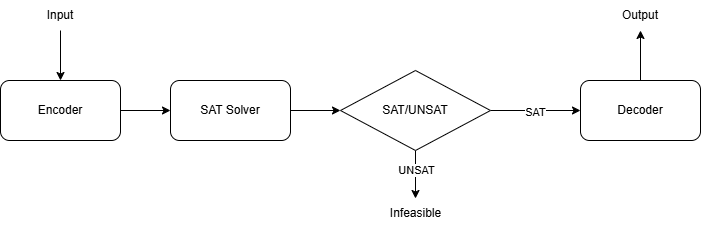
\includegraphics[width=0.72\linewidth]{figures/sat_flow.png}
    \caption{Overall execution pipeline of a modern SAT solver (SAT Solver Execution Flow).}
    \label{fig:sat_flow}
\end{figure}

As illustrated in Figure~\ref{fig:sat_flow}, the resolution pipeline starts with formalizing high-level constraints into propositional logic, encoding them into a CNF formula, passing them to the solver core, and extracting the corresponding solution assignment.

The state-of-the-art algorithmic framework implemented in modern industrial SAT solvers (e.g., Glucose4, MiniSat, Lingeling) is \textbf{Conflict-Driven Clause Learning (CDCL)} \cite{moskewicz2001chaff,audemard2009predicting,biere2010lingeling}. CDCL elevates classical DPLL search through key architectural pillars:
\begin{enumerate}
    \item \textbf{Unit Propagation (UP) and Two-Watched Literals (2WL):} Tracking exactly two unassigned literals per clause enables constant-time $O(1)$ propagation detection without iterating over entire clause contents.
    \item \textbf{Conflict Analysis and Learnt Clause Derivation:} When an assignment leads to a conflict (all literals in a clause evaluate to $\mathbf{False}$), the solver traverses the implication graph backward to the First-UIP (Unique Implication Point) cut to derive a learnt clause, preventing the solver from re-exploring identical conflict spaces.
    \item \textbf{Non-chronological Backjumping:} Directly jumping back across multiple decision levels to the highest safe assertion level following a conflict.
    \item \textbf{VSIDS (Variable State Independent Decaying Sum) Branching Heuristic:} Dynamically prioritizing branching on variables with high conflict participation frequencies, attenuated by an exponential decay factor.
    \item \textbf{LBD-based Clause Database Management:} Evaluating learnt clause quality using Literal Block Distance (the number of distinct decision levels in the clause); clauses with low LBD values are persistently retained in cache \cite{audemard2009predicting}.
\end{enumerate}

\subsection{SAT-based Encoding Concepts}
\label{subsec:sat_encoding_concept}
SAT encoding is the process of translating a high-level Constraint Satisfaction Problem (CSP) into an equisatisfiable CNF formula. An effective encoding must maintain an optimal balance across three dimensions:
\begin{itemize}
    \item \textbf{CNF Clause Count:} Maintaining linear or near-linear clause counts to prevent physical RAM exhaustion.
    \item \textbf{Auxiliary Variable Count:} Restricting auxiliary variables to avoid inflating the Boolean decision space explored by the solver's branching heuristic.
    \item \textbf{Preservation of Arc Consistency (GAC):} The capability to detect and prune conflicting assignments directly via Unit Propagation without requiring deep speculative branching.
\end{itemize}

\subsection{Optimized Encoding Methods for At-Most-One (AMO) Constraints}
\label{subsec:amo_encodings}
Given a set of $m$ Boolean variables $X = \{x_1, x_2, \dots, x_m\}$, the At-Most-One constraint enforces $\sum_{i=1}^m x_i \le 1$. Four advanced encoding techniques are investigated:

\subsubsection{Binary (Bitwise) Encoding}
Proposed by Frisch et al. \cite{frisch2005atmost}, this technique encodes the index of the $\mathbf{True}$ variable into binary bits:
\begin{itemize}
    \item Requires $k = \lceil \log_2 m \rceil$ auxiliary variables $b_1, b_2, \dots, b_k$.
    \item For each variable $x_i$, let the binary representation of $(i-1)$ be $d_1 d_2 \dots d_k \in \{0, 1\}^k$. If $x_i$ is $\mathbf{True}$, the auxiliary vector $(b_1, \dots, b_k)$ must match this binary codeword:
    \begin{equation}
    x_i \to \bigwedge_{j=1}^k (b_j = d_j) \iff \bigwedge_{j=1}^k (\neg x_i \lor l_{j, d_j})
    \end{equation}
    where $l_{j, 1} = b_j$ and $l_{j, 0} = \neg b_j$.
    \item Auxiliary variables: $O(\log m)$.
    \item Clauses: $m \lceil \log_2 m \rceil = O(m \log m)$.
\end{itemize}

\subsubsection{Sequential Counter Encoding}
Formulated by Carsten Sinz in 2005 \cite{sinz2005towards}, this technique mimics a hardware accumulator register counting the number of $\mathbf{True}$ assignments:
\begin{itemize}
    \item Introduces $m-1$ auxiliary variables $s_1, s_2, \dots, s_{m-1}$, where $s_i$ indicates that "at least one variable in the prefix $\{x_1, \dots, x_i\}$ is $\mathbf{True}$".
    \item The clause set consists of:
    \begin{align}
    (\neg x_1 \lor s_1) & \\
    (\neg s_{i-1} \lor s_i) & \quad \forall i \in [2, m-1] \quad \text{(State propagation)} \\
    (\neg x_i \lor s_i) & \quad \forall i \in [2, m-1] \quad \text{(State assignment)} \\
    (\neg s_{i-1} \lor \neg x_i) & \quad \forall i \in [2, m] \quad \text{(Conflict prevention)}
    \end{align}
    \item Auxiliary variables: $m - 1 = O(m)$.
    \item Clauses: $3m - 4 = O(m)$.
    \item Theoretical advantage: Strictly maintains Generalized Arc Consistency (GAC) through Unit Propagation.
\end{itemize}

\subsubsection{Commander Variable Encoding}
Klieber and Kwon (2007) \cite{klieber2007commander} proposed partitioning the variable set $X$ into small disjoint groups of size $g$ (typically $g=3$):
\begin{itemize}
    \item For each group $G_i$, a "commander variable" $c_i$ is introduced, which is $\mathbf{True}$ if and only if exactly one variable in $G_i$ is $\mathbf{True}$.
    \item Within each group $G_i$, local Pairwise encoding is applied ($\binom{g}{2} = 3$ clauses).
    \item An AMO constraint is recursively enforced across the set of commander variables $\{c_1, c_2, \dots, c_{\lceil m/g \rceil}\}$.
    \item Auxiliary variables: $O(m/g)$.
    \item Clauses: Linear $O(m)$.
\end{itemize}

\subsubsection{2-Product Matrix Encoding}
Jingchao Chen (2010) \cite{chen2010new} proposed mapping the set of $m$ variables onto a 2D grid of size $p \times q$ such that $p \times q \ge m$ (with $p \approx q \approx \lceil \sqrt{m} \rceil$):
\begin{itemize}
    \item Each variable $x_i$ is assigned a unique grid coordinate $(u, v)$ with $1 \le u \le p$ and $1 \le v \le q$.
    \item Introduces two sets of auxiliary variables: row variables $r_1, \dots, r_p$ and column variables $c_1, \dots, c_q$.
    \item If $x_i$ is $\mathbf{True}$, both row $r_u$ and column $c_v$ must be $\mathbf{True}$:
    \begin{equation}
    x_i \to r_u \land c_v \iff (\neg x_i \lor r_u) \land (\neg x_i \lor c_v)
    \end{equation}
    \item Enforces AMO on the row set $\{r_1, \dots, r_p\}$ and column set $\{c_1, \dots, c_q\}$.
    \item Auxiliary variables: $p + q = O(\sqrt{m})$.
    \item Clauses: $2m + O(p^2 + q^2) = O(m)$.
\end{itemize}

% =============================================================================
% SECTION 3: PROPOSED METHODOLOGY & MULTI-PARADIGM FORMULATION
% =============================================================================
\section{Proposed Methodology \& Multi-Paradigm Formulation}
\label{sec:methodology}

\subsection{Overview of the Methodology}
\label{subsec:method_overview}
To comprehensively evaluate exact solving methodologies on the $N$-Queens problem, two parallel research axes are deployed:
\begin{enumerate}
    \item \textbf{Axis 1 (SAT Solving):} Implementing and benchmarking five AMO encoding techniques: Binomial (Pairwise), Binary, Sequential Counter, Commander Variable ($g=3$), and 2-Product on an identical industrial SAT solver (PySAT Glucose4).
    \item \textbf{Axis 2 (Cross-Paradigm Comparison):} Directly pitting the top-performing SAT configuration against two baseline exact paradigms: Constraint Programming (Google OR-Tools CP-SAT, IBM ILOG CPLEX CP Optimizer) and 0-1 Mixed Integer Programming (Gurobi MIP, IBM ILOG CPLEX MIP).
\end{enumerate}

\subsection{Formulation of SAT Encodings for N-Queens}
\label{subsec:sat_encodings_nqueens}
The $N \times N$ chessboard is modeled with binary decision variables $B_{i,j}$ ($0 \le i, j < N$). The mathematical constraints are established as follows:

\paragraph{Row and Column Constraints:}
Each row $i$ and each column $j$ must contain exactly one queen:
\begin{align}
\text{ALO: } & \bigvee_{j=0}^{N-1} B_{i,j} \quad \forall i \in [0, N-1], \qquad \bigvee_{i=0}^{N-1} B_{i,j} \quad \forall j \in [0, N-1] \\
\text{AMO: } & \text{AMO}(B_{i,0}, \dots, B_{i,N-1}) \quad \forall i, \qquad \text{AMO}(B_{0,j}, \dots, B_{N-1,j}) \quad \forall j
\end{align}

\paragraph{Diagonal Constraints:}
The chessboard comprises $2N - 1$ main diagonals (index $k = i - j \in [-(N-1), N-1]$) and $2N - 1$ anti-diagonals (index $k = i + j \in [0, 2N-2]$). Because the single-square corner diagonals cannot contain conflicts, AMO constraints are applied strictly to diagonals with length $m \ge 2$:
\begin{align}
\text{Main diagonals: } & \text{AMO}(\{B_{i,j} \mid i - j = k\}), \quad \forall k \in [-(N-2), N-2] \\
\text{Anti-diagonals: } & \text{AMO}(\{B_{i,j} \mid i + j = k\}), \quad \forall k \in [1, 2N-3]
\end{align}

\subsection{Theoretical Complexity Comparison among 5 SAT Encodings}
\label{subsec:complexity_comparison}
Table~\ref{tab:encoding_complexity} summarizes the asymptotic complexity of the five encoding techniques for an AMO constraint of size $m$, as well as across the complete $N$-Queens problem instance.

\begin{table}[pos=htbp]
\centering
\caption{Theoretical complexity comparison of five SAT encoding methods on the $N$-Queens problem.}
\label{tab:encoding_complexity}
\begin{tabular}{lcccc}
\toprule
\textbf{Encoding Technique} & \textbf{\shortstack{Aux Vars\\/ AMO}} & \textbf{\shortstack{Clauses\\/ AMO}} & \textbf{\shortstack{Total\\Clauses}} & \textbf{\shortstack{Preserves\\GAC}} \\
\midrule
\textbf{Binomial (Pairwise)} & $0$ & $O(m^2)$ & $O(N^4)$ & Yes \\
\textbf{Sequential Counter}  & $O(m)$ & $O(m)$ & $O(N^2)$ & Yes \\
\textbf{Binary (Bitwise)}    & $O(\log m)$ & $O(m \log m)$ & $O(N^2 \log N)$ & No \\
\textbf{Commander Variable}  & $O(m/g)$ & $O(m)$ & $O(N^2)$ & No \\
\textbf{2-Product}           & $O(\sqrt{m})$ & $O(m)$ & $O(N^2)$ & No \\
\bottomrule
\end{tabular}
\end{table}

\subsection{Multi-Paradigm Formulations (CP and MIP)}
\label{subsec:cp_mip_formulations}

\subsubsection{Constraint Programming (CP) Model}
Constraint Programming provides the most compact and natural representation using $N$ integer decision variables $Q_0, Q_1, \dots, Q_{N-1}$ with domain $D(Q_i) = \{0, 1, \dots, N-1\}$, where $Q_i$ denotes the column coordinate of the queen placed on row $i$:
\begin{align}
\text{AllDifferent}(Q_0, Q_1, \dots, Q_{N-1}) & \quad \text{(Column conflict prevention)} \\
\text{AllDifferent}(Q_0 + 0, Q_1 + 1, \dots, Q_{N-1} + (N-1)) & \quad \text{(Anti-diagonal conflict prevention)} \\
\text{AllDifferent}(Q_0 - 0, Q_1 - 1, \dots, Q_{N-1} - (N-1)) & \quad \text{(Main diagonal conflict prevention)}
\end{align}
The entire formulation for an arbitrary scale $N$ requires only $N$ integer variables and exactly 3 global $\text{AllDifferent}$ constraints. IBM ILOG CPLEX CP Optimizer applies R{\'e}gin's propagation algorithm \cite{regin1994filtering} to perform domain filtering based on maximum bipartite matching.

\subsubsection{Mixed Integer Programming (MIP / 0-1 ILP) Model}
Mixed Integer Programming models the problem using $N^2$ binary decision variables $x_{i,j} \in \{0, 1\}$ analogous to SAT:
\begin{align}
\sum_{j=0}^{N-1} x_{i,j} &= 1 \quad \forall i \in [0, N-1] \quad \text{(Exactly one queen per row)} \\
\sum_{i=0}^{N-1} x_{i,j} &= 1 \quad \forall j \in [0, N-1] \quad \text{(Exactly one queen per column)} \\
\sum_{i-j=k} x_{i,j} &\le 1 \quad \forall k \in [-(N-2), N-2] \quad \text{(Main diagonals)} \\
\sum_{i+j=k} x_{i,j} &\le 1 \quad \forall k \in [1, 2N-3] \quad \text{(Anti-diagonals)}
\end{align}
The model consists of $N^2$ binary variables and $6N - 6$ linear equality and inequality constraints, solved via Branch-and-Cut incorporating polyhedral cutting planes and continuous Simplex LP relaxation.

% =============================================================================
% SECTION 4: COMPUTATIONAL EXPERIMENTS
% =============================================================================
\section{Computational Experiments and Results}
\label{sec:experiments}

\subsection{Benchmark Settings and Dataset}
\label{subsec:dataset_settings}
To rigorously assess scalability, the benchmark suite is standardized across 15 problem instances:
\begin{equation}
N \in \{4, 8, 16, 25, 36, 49, 64, 81, 100, 125, 216, 343, 512, 729, 1000\}
\end{equation}
The largest instance $N = 1000$ represents an ultra-scale benchmark comprising $1,000,000$ decision variables and approximately $14,000,000$ CNF clauses. A strict execution timeout of \textbf{$120.0$ seconds} is enforced per run. Instances exceeding this limit are marked as \texttt{TIMEOUT}. Instances whose formula generation exceeds 16 GB RAM are designated as \texttt{SKIPPED\_MEMLIMIT} to maintain system integrity.

\subsection{Experimental Environment}
\label{subsec:exp_env}
Detailed specifications of the hardware platform and software solvers are standardized in Table~\ref{tab:env_config}.

\begin{table}[pos=htbp]
\centering
\caption{Hardware platform and software solver environment specifications.}
\label{tab:env_config}
\begin{tabularx}{\textwidth}{>{\raggedright\arraybackslash}p{4.8cm} X}
\toprule
\textbf{Specification Parameter} & \textbf{Configuration Details} \\
\midrule
Processor (CPU) & 12th Gen Intel(R) Core(TM) i5-14500H (12 cores, 8 threads, up to 4.4 GHz) \\
System Memory (RAM) & 16.0 GB DDR4 \\
Operating System & Ubuntu 26.04 LTS (Linux x86\_64) \\
Execution Environment & Python 3.14.4 \\
SAT Solver & PySAT v1.9.dev15 (Solver core: Glucose4) \\
CP Solver (Hybrid Engine) & Google OR-Tools v9.15.6755 (CP-SAT Solver) \\
CP Solver (Pure CP Engine) & IBM ILOG CPLEX Optimization Studio v22.1.1 (CP Optimizer) \\
MIP Solver 1 & Gurobi Optimizer v13.0.3 (Academic License) \\
MIP Solver 2 & IBM ILOG CPLEX Optimization Studio v22.1.1 (MIP Academic License) \\
\bottomrule
\end{tabularx}
\end{table}

\subsection{Empirical Evaluation of the 5 SAT Encodings}
\label{subsec:sat_enc_results}
Table~\ref{tab:sat_encodings_runtime} compares the execution runtimes (seconds) of the five SAT encodings on Glucose4 across all 15 benchmark sizes. Comprehensive empirical measurements encompassing variable and clause counts are compiled in Appendix~\ref{app:detailed_data}.

\begin{table}[pos=htbp]
\centering
\caption{Execution runtime (seconds) of five SAT encoding techniques on the Glucose4 solver across 15 problem instances ($N \in [4, 1000]$).}
\label{tab:sat_encodings_runtime}
\begin{tabular}{rrrrrr}
\toprule
$N$ & \textbf{Binomial} & \textbf{Binary} & \textbf{Sequential} & \textbf{Commander} & \textbf{2-Product} \\
\midrule
4    & 0.00039 & 0.00041 & 0.00032 & \textbf{0.00021} & 0.00034 \\
8    & 0.00079 & 0.00075 & 0.00077 & 0.00081 & \textbf{0.00072} \\
16   & 0.01094 & 0.02093 & \textbf{0.00600} & 0.01760 & 0.10392 \\
25   & \textbf{0.00916} & 0.05290 & 0.06090 & 0.17529 & 0.14078 \\
36   & \textbf{0.02714} & 0.05251 & 0.16478 & 0.04235 & 7.73743 \\
49   & 0.08398 & \textbf{0.05116} & 1.14570 & 0.83751 & 10.47424 \\
64   & 0.18140 & 0.13639 & 1.65263 & \textbf{0.06721} & 12.07009 \\
81   & 0.35869 & \textbf{0.11759} & 24.01935 & 0.27075 & 15.55798 \\
100  & 0.68852 & \textbf{0.14738} & 46.52458 & 0.16474 & 15.32860 \\
125  & 1.29502 & \textbf{0.24989} & 45.29085 & 0.61935 & 25.38504 \\
216  & 6.03935 & \textbf{0.81394} & 89.66358 & 1.29397 & 41.69153 \\
343  & 19.89517 & 2.31824 & \texttt{TIMEOUT} & \textbf{2.09605} & 69.55248 \\
512  & \texttt{MEMLIMIT} & \textbf{5.44507} & \texttt{TIMEOUT} & 6.67240 & \texttt{TIMEOUT} \\
729  & \texttt{MEMLIMIT} & 64.82834 & \texttt{TIMEOUT} & \textbf{28.44704} & \texttt{TIMEOUT} \\
1000 & \texttt{MEMLIMIT} & 24.66207 & \texttt{TIMEOUT} & \textbf{20.09668} & \texttt{TIMEOUT} \\
\bottomrule
\end{tabular}
\end{table}

\begin{figure}[pos=htbp]
    \centering
    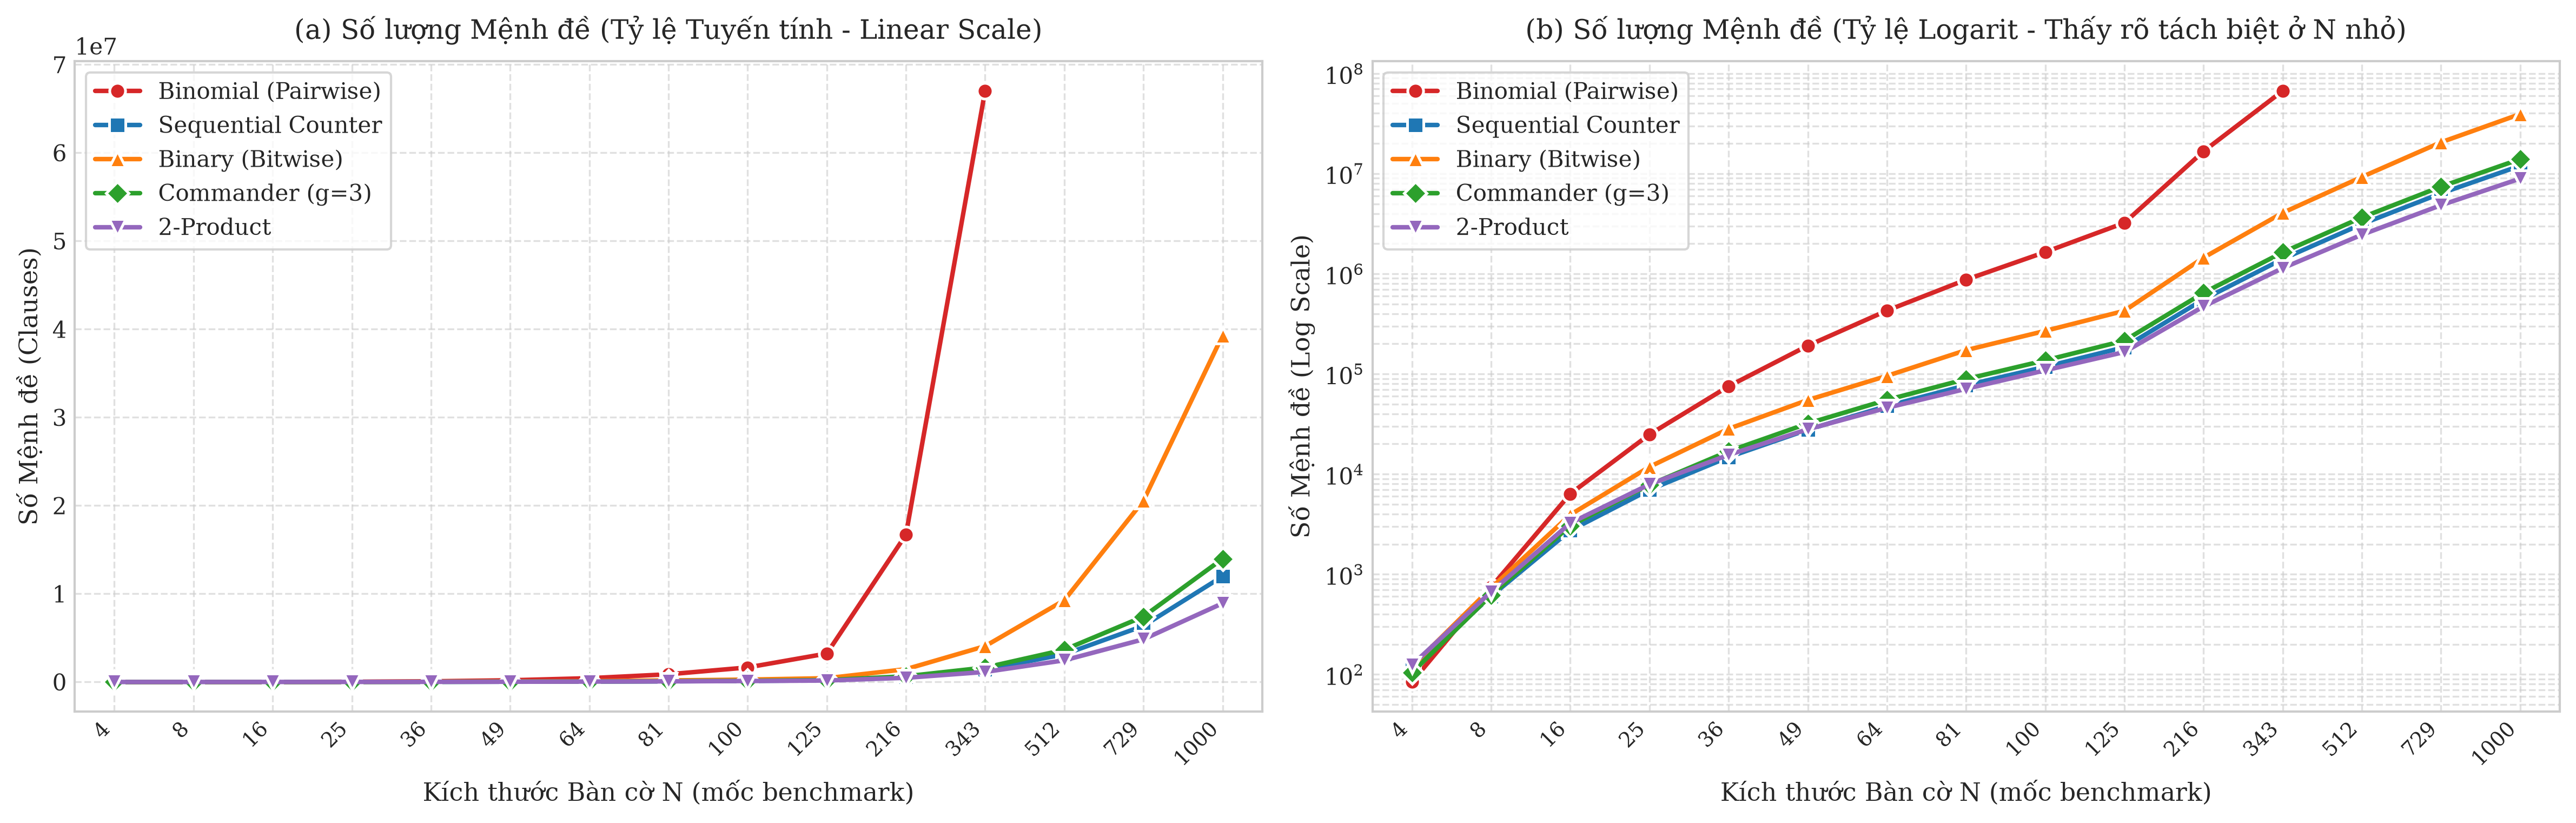
\includegraphics[width=0.92\linewidth]{figures/encoding_clauses.png}
    \caption{Comparison of generated CNF clause counts among five SAT encodings across 15 problem instances ($N \in [4, 1000]$) on linear scale (left) and logarithmic scale (right).}
    \label{fig:enc_clauses}
\end{figure}

\begin{figure}[pos=htbp]
    \centering
    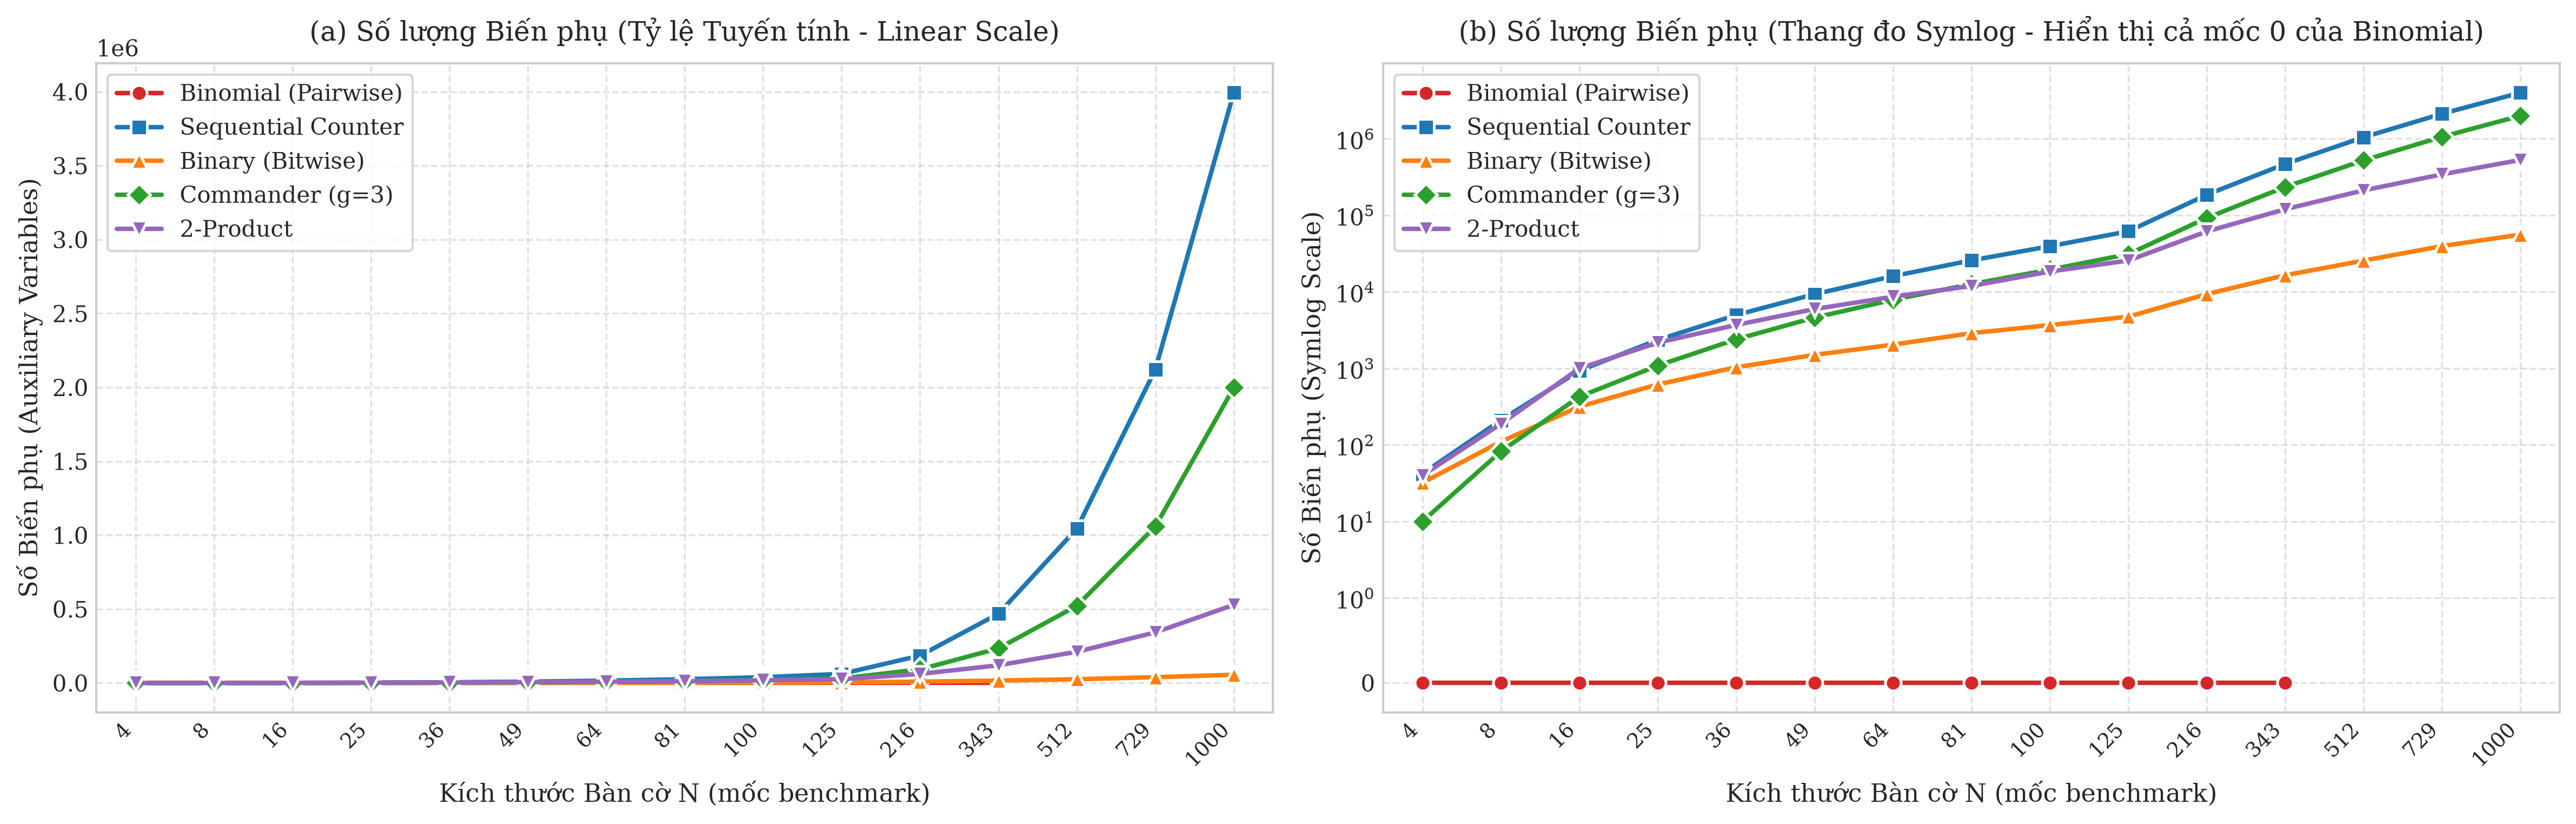
\includegraphics[width=0.92\linewidth]{figures/encoding_aux_vars.png}
    \caption{Comparison of auxiliary variable counts among five SAT encodings across 15 problem instances ($N \in [4, 1000]$) on linear scale (left) and symmetric log scale (right).}
    \label{fig:enc_aux_vars}
\end{figure}

\begin{figure}[pos=htbp]
    \centering
    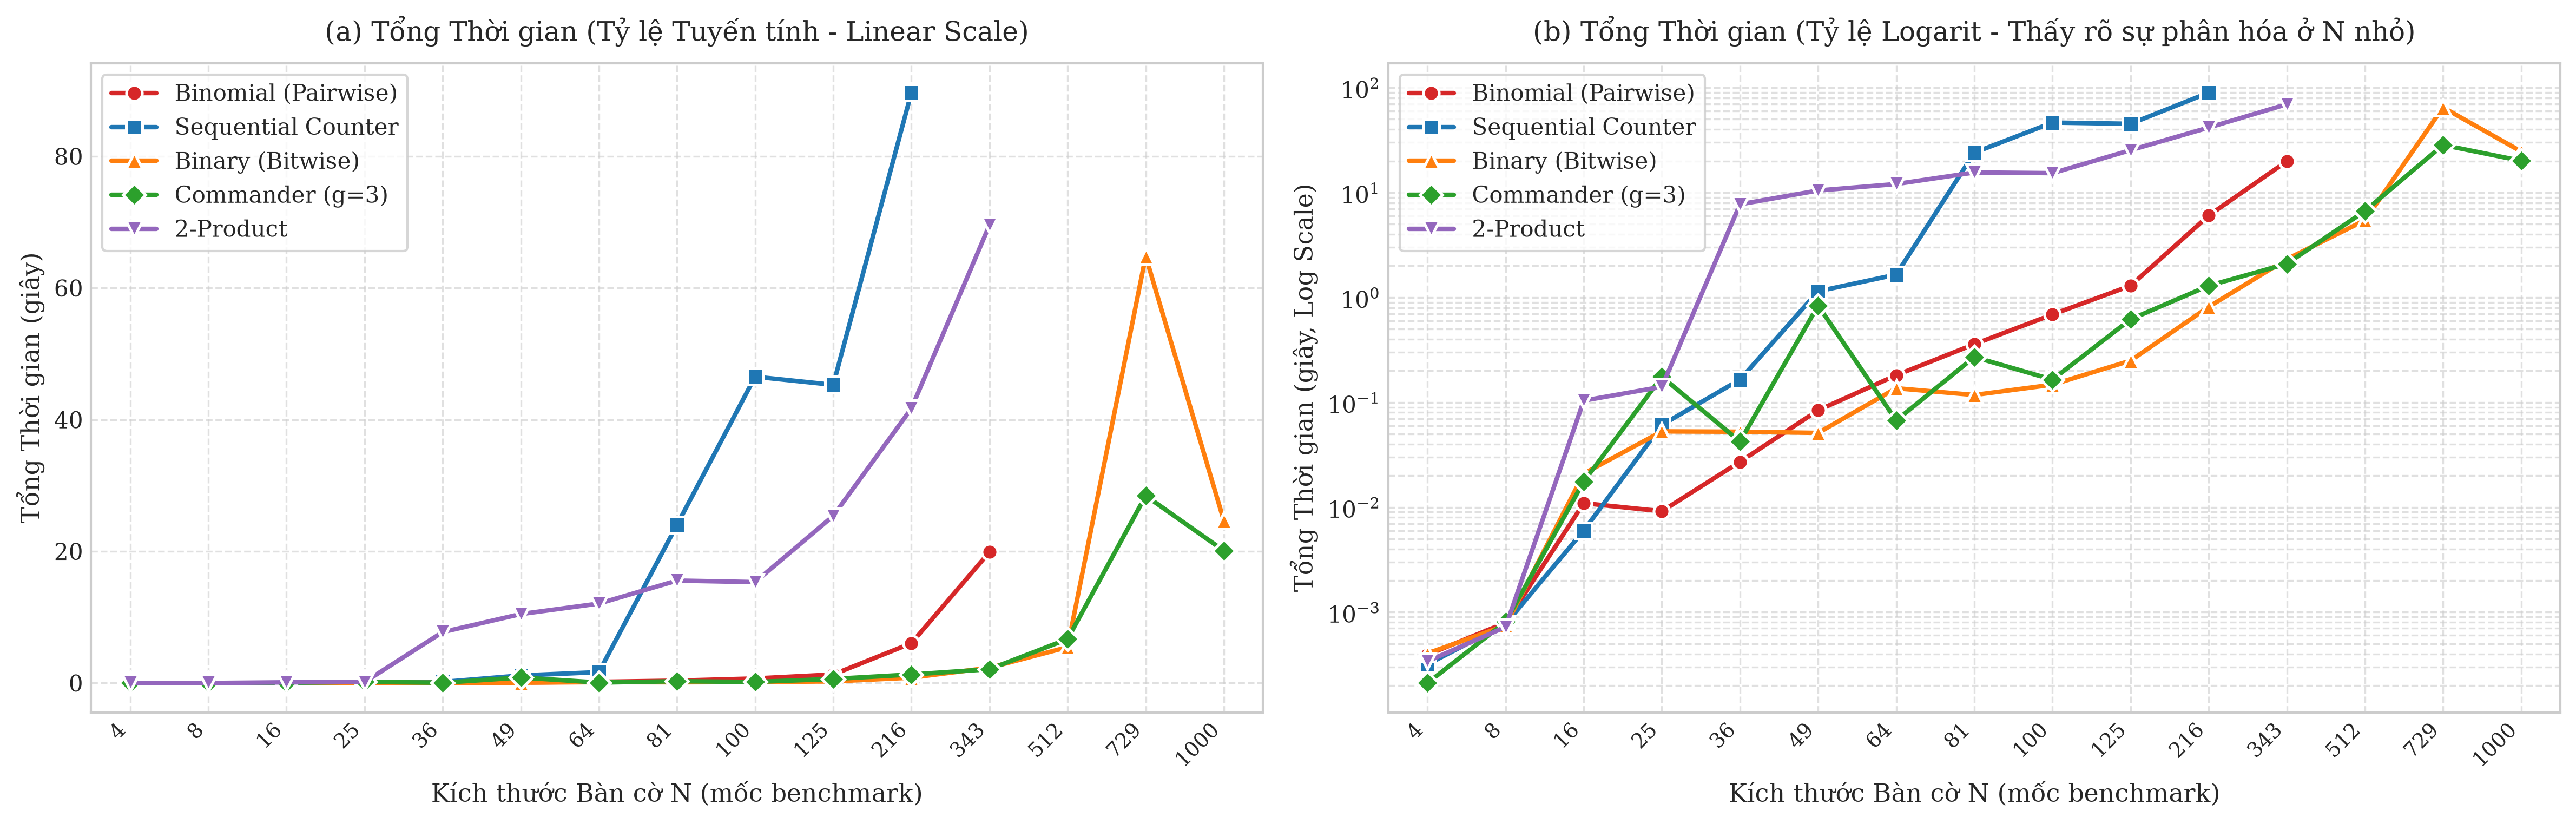
\includegraphics[width=0.92\linewidth]{figures/encoding_total_time.png}
    \caption{Comparison of total execution runtime among five SAT encodings on the Glucose4 solver across 15 problem instances ($N \in [4, 1000]$) on linear scale (left) and logarithmic scale (right).}
    \label{fig:enc_time}
\end{figure}

\subsection{In-Depth Empirical Analysis}
\label{subsec:deep_analysis}

\paragraph{1. Quartic Clause Explosion in Binomial Encoding:}
The Binomial encoding delivers exceptional solving speed on small matrices ($N \le 25$) because it introduces zero auxiliary variables ($0$ auxiliary variables). However, the quartic growth $O(N^4)$ in clause count rapidly reveals severe limitations:
\begin{itemize}
    \item At $N = 100$, Binomial generates over $1.64$ million clauses.
    \item At $N = 343$, the clause count surges past $67.0$ million clauses, requiring $5.09$ seconds simply to construct the formula and $14.80$ seconds to solve it.
    \item At $N \ge 512$, formula generation exceeds 16 GB of physical RAM, triggering an Out-Of-Memory error (\texttt{SKIPPED\_MEMLIMIT}).
\end{itemize}

\paragraph{2. The Sequential Counter Paradox:}
Theoretically, Sequential Counter is considered an ideal encoding because it maintains a linear clause complexity $O(m)$ while strictly preserving Generalized Arc Consistency (GAC) through Unit Propagation \cite{sinz2005towards}. However, empirical evidence reveals that it performs worst at scale, suffering a \texttt{TIMEOUT} starting from $N = 343$. The fundamental cause of this paradox lies in the severe disruption caused by auxiliary variables to the CDCL solver's branching mechanisms:
\begin{enumerate}
    \item At $N = 1000$, Sequential Counter introduces $3,994,002$ auxiliary variables---nearly 4 times the number of original decision variables ($1,000,000$).
    \item The state propagation clauses $(\neg s_{i-1} \lor s_i)$ heavily populate the solver's unit propagation chains and implication graph. The VSIDS heuristic continually boosts the activity scores of these internal register variables $s_i$, misleading the solver into selecting auxiliary variables for branching decisions.
    \item Branching on an internal accumulator variable $s_i$ provides negligible search-space pruning compared to branching directly on an original board variable $B_{i,j}$, leading to search thrashing and an explosion in the search tree depth.
\end{enumerate}

\paragraph{3. Superiority of Binary and Commander Variable Encodings:}
\begin{itemize}
    \item \textbf{Binary (Bitwise):} Demonstrates the most parsimonious auxiliary variable footprint (only $55,888$ auxiliary variables at $N = 1000$, representing less than $5.6\%$ of original decision variables). Preserving a compact variable space enables VSIDS to remain focused on primary board variables, achieving leading performance in the mid-range $N \in [49, 216]$ ($0.81$s at $N=216$) and successfully solving all 15 instances up to $N = 1000$ in $24.66$ seconds.
    \item \textbf{Commander Variable ($g=3$):} Achieves the optimal trade-off between reducing clause counts and controlling auxiliary variable expansion. Commander is the fastest SAT encoding at extreme scale $N \ge 343$: completing $N = 343$ in $2.10$s, $N = 729$ in $28.45$s (over $2\times$ faster than Binary's $64.83$s), and solving $N = 1000$ in only $20.10$ seconds.
\end{itemize}

\subsection{Cross-Paradigm Benchmark (SAT vs CP vs MIP)}
\label{subsec:cross_paradigm_results}
Table~\ref{tab:cross_paradigm_results} presents the head-to-head performance of the best-performing SAT configuration (PySAT Glucose4 Commander) against four industrial CP and MIP solvers across the 15 benchmark instances.

\begin{table}[pos=htbp]
\centering
\caption{Cross-paradigm runtime benchmark (seconds) across three exact solving paradigms: SAT (Glucose4 Commander), Constraint Programming CP (OR-Tools, CPLEX CP), and Mixed Integer Programming MIP (Gurobi, CPLEX MIP) across 15 problem instances ($N \in [4, 1000]$).}
\label{tab:cross_paradigm_results}
\small
\setlength{\tabcolsep}{4pt}
\begin{tabular}{rrrrrr}
\toprule
$N$ & \textbf{\shortstack{PySAT\\(SAT)}} & \textbf{\shortstack{OR-Tools\\(CP)}} & \textbf{\shortstack{CPLEX\\(CP)}} & \textbf{\shortstack{Gurobi\\(MIP)}} & \textbf{\shortstack{CPLEX\\(MIP)}} \\
\midrule
4    & \textbf{0.00035} & 0.00693 & 0.01040 & 0.00144 & 0.02712 \\
8    & 0.00092 & 0.00484 & 0.00860 & \textbf{0.00075} & 0.01483 \\
16   & 0.01730 & 0.01142 & 0.00836 & \textbf{0.00782} & 0.01695 \\
25   & 0.17280 & 0.03455 & 0.01455 & \textbf{0.00247} & 0.02269 \\
36   & 0.03943 & 0.03944 & \textbf{0.01124} & 0.01598 & 0.03602 \\
49   & 0.81583 & 0.07143 & 0.01096 & \textbf{0.00850} & 0.04459 \\
64   & 0.06577 & 0.14754 & 0.01125 & \textbf{0.01115} & 0.07155 \\
81   & 0.28050 & 0.27732 & \textbf{0.01325} & 0.01780 & 0.09460 \\
100  & 0.17549 & 0.44541 & \textbf{0.01423} & 0.03066 & 0.12695 \\
125  & 0.66580 & 0.79482 & \textbf{0.01832} & 0.04310 & 0.20795 \\
216  & 1.27169 & 9.93486 & \textbf{0.02089} & 0.14242 & 0.66035 \\
343  & 2.13944 & 79.70357 & \textbf{0.03815} & 0.36060 & 1.94325 \\
512  & 6.29781 & \texttt{TIMEOUT} & \textbf{0.07285} & 0.83847 & 4.98140 \\
729  & 28.49975 & \texttt{TIMEOUT} & \textbf{0.12560} & 24.10297 & 14.90481 \\
1000 & 18.91856 & \texttt{TIMEOUT} & \textbf{0.25016} & \texttt{TIMEOUT} & 19.41587 \\
\bottomrule
\end{tabular}
\end{table}

\begin{figure}[pos=htbp]
    \centering
    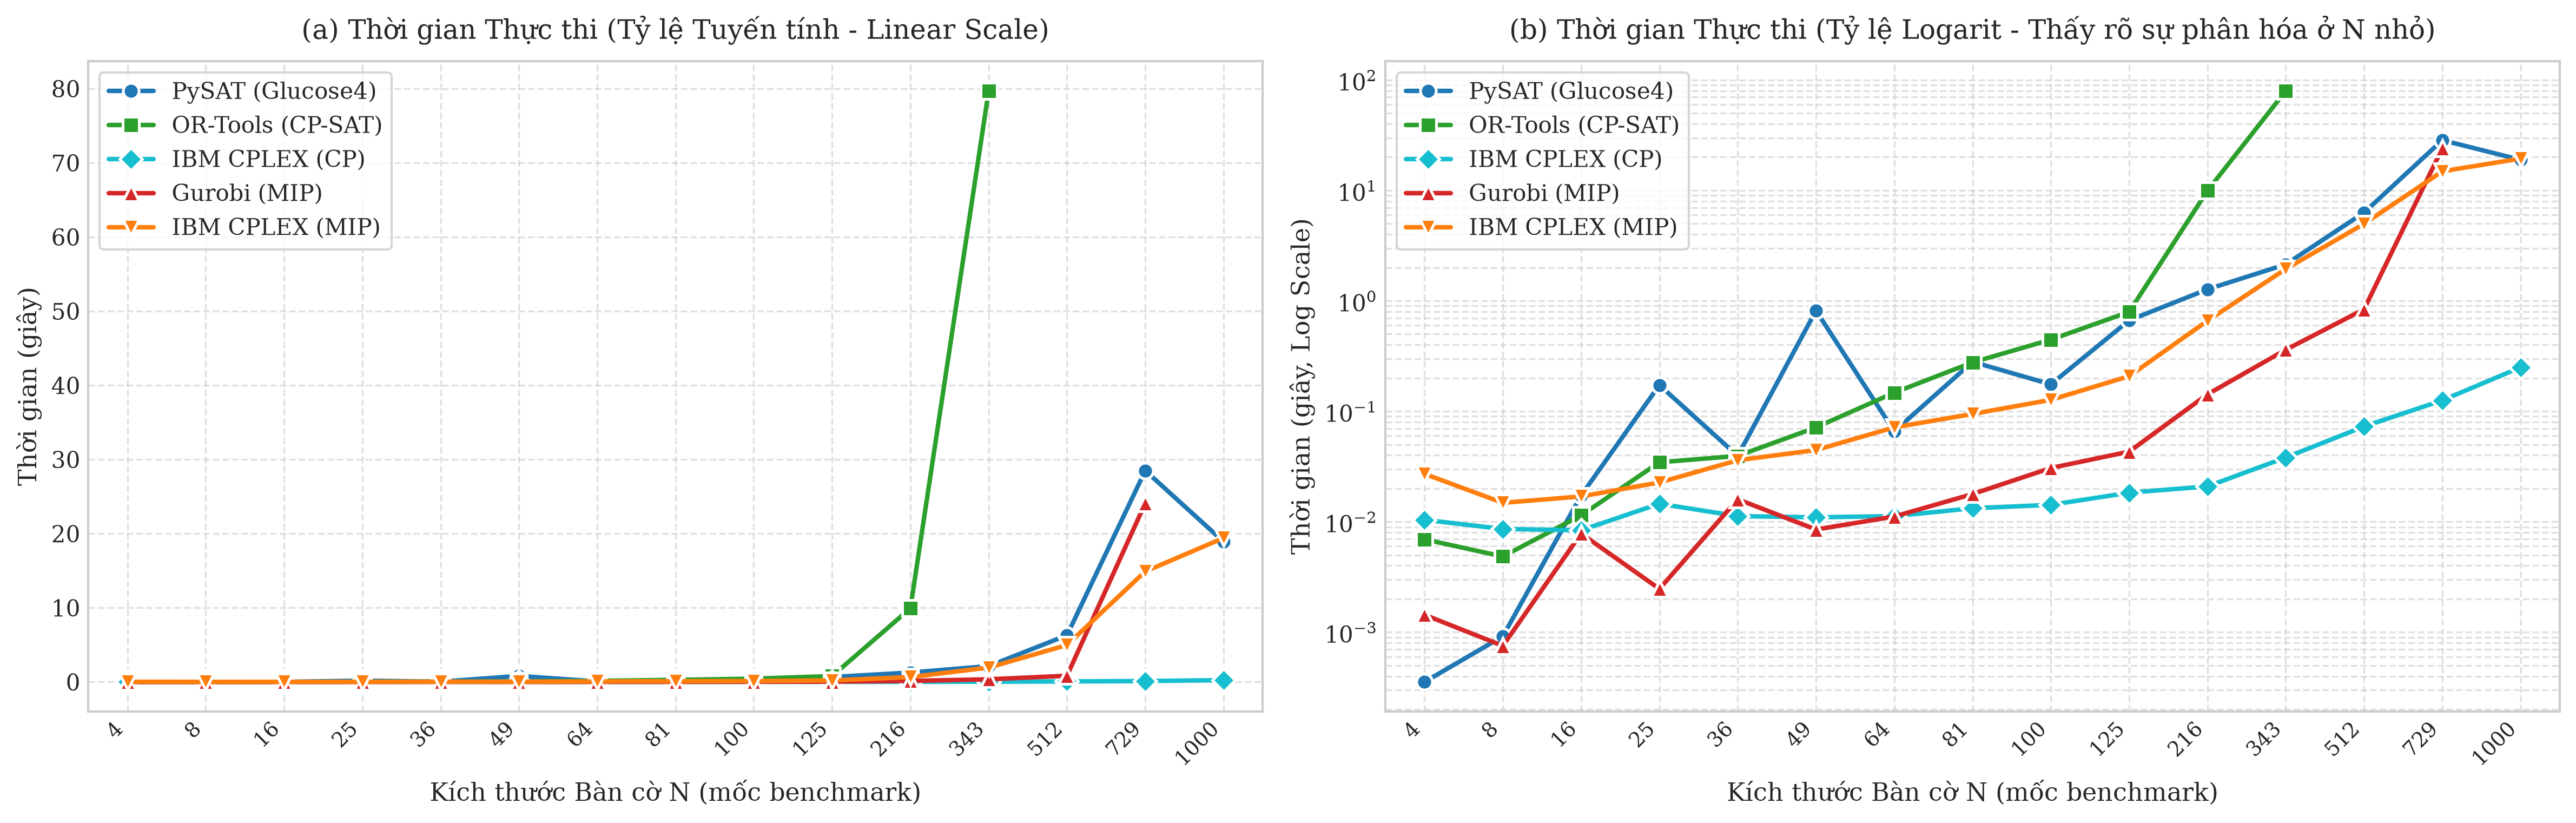
\includegraphics[width=0.92\linewidth]{figures/solver_total_time.png}
    \caption{Multi-paradigm runtime comparison (linear scale on the left, logarithmic scale on the right) among SAT (PySAT Glucose4 Commander), Constraint Programming CP (Google OR-Tools CP-SAT, IBM CPLEX CP), and Mixed Integer Programming MIP (Gurobi MIP, IBM CPLEX MIP) across 15 problem instances ($N \in [4, 1000]$).}
    \label{fig:solver_time}
\end{figure}

\paragraph{Detailed Discussion on Multi-Paradigm Performance:}
\begin{enumerate}
    \item \textbf{IBM CPLEX CP Optimizer:} Leveraging a compact representation with only $N$ integer variables and 3 global $\text{AllDifferent}$ constraints, coupled with R{\'e}gin's bipartite matching filtering algorithm, CPLEX CP maintains solve times below $0.04$ seconds for all $N \le 343$, and solves the $N = 1000$ chessboard in merely \textbf{$0.250$ seconds}. It represents the unconditionally dominant technology for the $N$-Queens problem.
    \item \textbf{IBM CPLEX MIP:} Equipped with a full academic license, CPLEX MIP successfully solves the $N = 1000$ instance ($1,000,000$ binary variables) in \textbf{$19.42$ seconds}, demonstrating the power of IBM's advanced Presolve routines and polyhedral Branch-and-Cut cuts.
    \item \textbf{Gurobi Optimizer (MIP):} Gurobi delivers remarkable performance up to $N = 729$: $N = 512$ ($262,144$ variables) in $0.838$ seconds, and $N = 729$ ($531,441$ variables) in $24.10$ seconds. However, at $N = 1000$, the expanding Branch-and-Bound search space causes the solver to hit the \texttt{TIMEOUT} limit (120s).
    \item \textbf{PySAT Glucose4 (Commander Variable):} Glucose4 with Commander Variable encoding successfully completes all 15 instances up to $N = 1000$ in \textbf{$18.92$ seconds} (in the solver benchmark) and $20.10$ seconds (in the encoding benchmark). Remarkably, Glucose4 outperforms both Gurobi and OR-Tools CP-SAT at $N = 1000$, demonstrating that modern CDCL SAT solvers are fully capable of solving million-variable problems when equipped with optimized encoding techniques.
    \item \textbf{Google OR-Tools (CP-SAT):} Demonstrates competitive performance for $N \le 343$ ($79.70$ seconds), but encounters \texttt{TIMEOUT} at $N \ge 512$ due to internal Boolean flattening of global constraints, which induces search thrashing similar to the Sequential Counter encoding.
\end{enumerate}

% =============================================================================
% SECTION 5: CONCLUSION
% =============================================================================
\section{Conclusion}
\label{sec:conclusion}

\subsection{Summary of Findings}
\label{subsec:conclusion_summary}
This study has presented an extensive theoretical and empirical investigation of the $N$-Queens problem across exact computing paradigms:
\begin{enumerate}
    \item Thoroughly benchmarked five At-Most-One (AMO) SAT encodings: Unveiled the quartic clause explosion of Binomial encoding causing physical RAM exhaustion at $N \ge 512$, and elucidated the \textit{Sequential Counter Paradox}, where millions of auxiliary variables dilute the CDCL solver's VSIDS branching heuristic.
    \item Established the superiority of \textbf{Binary Encoding} in auxiliary variable parsimony ($55.9\text{K}$ variables at $N=1000$, fastest for $N \in [49, 216]$) and the balanced efficiency of \textbf{Commander Variable Encoding} (fastest for $N \ge 343$, solving $N = 1000$ in $18.92$s).
    \item Conducted a rigorous cross-paradigm benchmark between SAT, CP, and MIP across 15 synchronized instances up to $N = 1000$.
\end{enumerate}

\subsection{Technology Selection Recommendations}
\label{subsec:recommendations}
Based on our quantitative empirical analyses, we provide practical recommendations for technology selection:
\begin{itemize}
    \item \textbf{For pure constraint satisfaction problems at ultra-large scale ($N \ge 500$):} \textbf{Constraint Programming (IBM CPLEX CP Optimizer)} is the premier solution, offering sub-second response times ($0.25\text{s}$ for $N = 1000$).
    \item \textbf{For 0-1 Boolean binary formulations:} \textbf{PySAT Glucose4 (Commander Variable)} and \textbf{IBM CPLEX MIP} are the two standout solvers, demonstrating the capacity to solve million-variable instances within 20 seconds without memory bottlenecks.
\end{itemize}

% -----------------------------------------------------------------------------
% DATA AVAILABILITY
% -----------------------------------------------------------------------------
\section*{Data availability}
All algorithm source code implementations (five SAT encodings, four baseline CP and MIP models), automated benchmark execution scripts, comprehensive empirical datasets (CSV format), and visualization scripts are publicly accessible at the author's GitHub repository: \url{https://github.com/NhHung07/N_Queens.git}.

% -----------------------------------------------------------------------------
% APPENDIX
% -----------------------------------------------------------------------------
\appendix
\section{Comprehensive Detailed Experimental Data of 5 SAT Encodings}
\label{app:detailed_data}

Below is the complete, detailed empirical measurement dataset of the five At-Most-One (AMO) encoding techniques evaluated on PySAT Glucose4 across 15 problem instances ($N \in [4, 1000]$).

\begingroup
\scriptsize
\setlength{\tabcolsep}{2.5pt}
\begin{longtable}{r l r r r r r r c}
\caption{Complete empirical measurement data of five SAT encoding techniques on PySAT Glucose4 across 15 problem instances.} \label{tab:full_sat_data} \\
\toprule
$N$ & \textbf{Technique} & \textbf{\shortstack{Total\\Vars}} & \textbf{\shortstack{Aux\\Vars}} & \textbf{\shortstack{Clause\\Count}} & \textbf{\shortstack{Gen Time\\(s)}} & \textbf{\shortstack{Solve Time\\(s)}} & \textbf{\shortstack{Total Time\\(s)}} & \textbf{Status} \\
\midrule
\endfirsthead

\multicolumn{9}{c}{\tablename\ \thetable\ -- Continued from previous page} \\
\toprule
$N$ & \textbf{Technique} & \textbf{\shortstack{Total\\Vars}} & \textbf{\shortstack{Aux\\Vars}} & \textbf{\shortstack{Clause\\Count}} & \textbf{\shortstack{Gen Time\\(s)}} & \textbf{\shortstack{Solve Time\\(s)}} & \textbf{\shortstack{Total Time\\(s)}} & \textbf{Status} \\
\midrule
\endhead

\midrule
\multicolumn{9}{r}{Continued on next page \dots} \\
\bottomrule
\endfoot

\bottomrule
\endlastfoot

\multirow{5}{*}{4} 
 & Binomial & 16 & 0 & 84 & 0.000031 & 0.000361 & 0.000393 & \texttt{SAT} \\
 & Sequential & 58 & 42 & 116 & 0.000033 & 0.000285 & 0.000318 & \texttt{SAT} \\
 & Binary & 48 & 32 & 120 & 0.000065 & 0.000339 & 0.000405 & \texttt{SAT} \\
 & Commander & 26 & 10 & 104 & 0.000040 & 0.000171 & \textbf{0.000211} & \texttt{SAT} \\
 & 2-Product & 56 & 40 & 124 & 0.000059 & 0.000281 & 0.000340 & \texttt{SAT} \\
\midrule
\multirow{5}{*}{8} 
 & Binomial & 64 & 0 & 744 & 0.000171 & 0.000622 & 0.000792 & \texttt{SAT} \\
 & Sequential & 274 & 210 & 604 & 0.000089 & 0.000684 & 0.000773 & \texttt{SAT} \\
 & Binary & 174 & 110 & 728 & 0.000144 & 0.000603 & 0.000746 & \texttt{SAT} \\
 & Commander & 146 & 82 & 618 & 0.000122 & 0.000686 & 0.000808 & \texttt{SAT} \\
 & 2-Product & 252 & 188 & 668 & 0.000109 & 0.000614 & \textbf{0.000723} & \texttt{SAT} \\
\midrule
\multirow{5}{*}{16} 
 & Binomial & 256 & 0 & 6,352 & 0.000570 & 0.010369 & 0.010939 & \texttt{SAT} \\
 & Sequential & 1,186 & 930 & 2,732 & 0.000194 & 0.005807 & \textbf{0.006000} & \texttt{SAT} \\
 & Binary & 572 & 316 & 3,928 & 0.000453 & 0.020475 & 0.020928 & \texttt{SAT} \\
 & Commander & 682 & 426 & 3,052 & 0.000424 & 0.017172 & 0.017596 & \texttt{SAT} \\
 & 2-Product & 1,252 & 996 & 3,236 & 0.000426 & 0.103495 & 0.103921 & \texttt{SAT} \\
\midrule
\multirow{5}{*}{25} 
 & Binomial & 625 & 0 & 24,850 & 0.001967 & 0.007194 & \textbf{0.009161} & \texttt{SAT} \\
 & Sequential & 2,977 & 2,352 & 6,962 & 0.000503 & 0.060392 & 0.060895 & \texttt{SAT} \\
 & Binary & 1,241 & 616 & 11,806 & 0.001082 & 0.051813 & 0.052895 & \texttt{SAT} \\
 & Commander & 1,709 & 1,084 & 7,810 & 0.001046 & 0.174248 & 0.175294 & \texttt{SAT} \\
 & 2-Product & 2,789 & 2,164 & 7,894 & 0.000722 & 0.140053 & 0.140775 & \texttt{SAT} \\
\midrule
\multirow{5}{*}{36} 
 & Binomial & 1,296 & 0 & 75,252 & 0.006442 & 0.020699 & \textbf{0.027140} & \texttt{SAT} \\
 & Sequential & 6,266 & 4,970 & 14,772 & 0.001122 & 0.163660 & 0.164782 & \texttt{SAT} \\
 & Binary & 2,328 & 1,032 & 28,320 & 0.002558 & 0.049948 & 0.052506 & \texttt{SAT} \\
 & Commander & 3,690 & 2,394 & 16,904 & 0.002307 & 0.040042 & 0.042349 & \texttt{SAT} \\
 & 2-Product & 4,988 & 3,692 & 15,548 & 0.001730 & 7.735702 & 7.737431 & \texttt{SAT} \\
\midrule
\multirow{5}{*}{49} 
 & Binomial & 2,401 & 0 & 191,394 & 0.030131 & 0.053853 & 0.083984 & \texttt{SAT} \\
 & Sequential & 11,713 & 9,312 & 27,746 & 0.012348 & 1.133353 & 1.145701 & \texttt{SAT} \\
 & Binary & 3,901 & 1,500 & 54,866 & 0.005207 & 0.045954 & \textbf{0.051161} & \texttt{SAT} \\
 & Commander & 7,009 & 4,608 & 32,014 & 0.003766 & 0.833742 & 0.837507 & \texttt{SAT} \\
 & 2-Product & 8,353 & 5,952 & 27,998 & 0.002204 & 10.472035 & 10.474239 & \texttt{SAT} \\
\midrule
\multirow{5}{*}{64} 
 & Binomial & 4,096 & 0 & 428,864 & 0.068978 & 0.112422 & 0.181400 & \texttt{SAT} \\
 & Sequential & 20,098 & 16,002 & 47,756 & 0.002972 & 1.649655 & 1.652627 & \texttt{SAT} \\
 & Binary & 6,136 & 2,040 & 95,576 & 0.011644 & 0.124750 & 0.136394 & \texttt{SAT} \\
 & Commander & 11,958 & 7,862 & 55,022 & 0.014461 & 0.052746 & \textbf{0.067207} & \texttt{SAT} \\
 & 2-Product & 12,732 & 8,636 & 45,876 & 0.003465 & 12.066623 & 12.070088 & \texttt{SAT} \\
\midrule
\multirow{5}{*}{81} 
 & Binomial & 6,561 & 0 & 872,802 & 0.149942 & 0.208745 & 0.358687 & \texttt{SAT} \\
 & Sequential & 32,321 & 25,760 & 76,962 & 0.005572 & 24.013778 & 24.019350 & \texttt{SAT} \\
 & Binary & 9,441 & 2,880 & 172,694 & 0.034938 & 0.082653 & \textbf{0.117590} & \texttt{SAT} \\
 & Commander & 19,177 & 12,616 & 88,778 & 0.013516 & 0.257236 & 0.270753 & \texttt{SAT} \\
 & 2-Product & 18,477 & 11,916 & 70,966 & 0.015049 & 15.542931 & 15.557980 & \texttt{SAT} \\
\midrule
\multirow{5}{*}{100} 
 & Binomial & 10,000 & 0 & 1,646,900 & 0.300462 & 0.388057 & 0.688519 & \texttt{SAT} \\
 & Sequential & 49,402 & 39,402 & 117,812 & 0.011384 & 46.513192 & 46.524576 & \texttt{SAT} \\
 & Binary & 13,678 & 3,678 & 269,024 & 0.051690 & 0.095692 & \textbf{0.147383} & \texttt{SAT} \\
 & Commander & 29,502 & 19,502 & 136,560 & 0.030482 & 0.134258 & 0.164740 & \texttt{SAT} \\
 & 2-Product & 28,408 & 18,408 & 108,596 & 0.010247 & 15.318352 & 15.328598 & \texttt{SAT} \\
\midrule
\multirow{5}{*}{125} 
 & Binomial & 15,625 & 0 & 3,224,250 & 0.509696 & 0.785323 & 1.295019 & \texttt{SAT} \\
 & Sequential & 77,377 & 61,752 & 184,762 & 0.024211 & 45.266639 & 45.290850 & \texttt{SAT} \\
 & Binary & 20,353 & 4,728 & 426,574 & 0.078129 & 0.171765 & \textbf{0.249894} & \texttt{SAT} \\
 & Commander & 46,685 & 31,060 & 214,918 & 0.041198 & 0.578150 & 0.619348 & \texttt{SAT} \\
 & 2-Product & 41,253 & 25,628 & 165,386 & 0.017037 & 25.367998 & 25.385035 & \texttt{SAT} \\
\midrule
\multirow{5}{*}{216} 
 & Binomial & 46,656 & 0 & 16,703,352 & 2.188771 & 3.850577 & 6.039348 & \texttt{SAT} \\
 & Sequential & 231,986 & 185,330 & 555,132 & 0.108629 & 89.554950 & 89.663579 & \texttt{SAT} \\
 & Binary & 55,988 & 9,332 & 1,449,224 & 0.278691 & 0.535247 & \textbf{0.813938} & \texttt{SAT} \\
 & Commander & 139,002 & 92,346 & 645,382 & 0.161277 & 1.132691 & 1.293968 & \texttt{SAT} \\
 & 2-Product & 108,096 & 61,440 & 471,448 & 0.060232 & 41.631297 & 41.691528 & \texttt{SAT} \\
\midrule
\multirow{5}{*}{343} 
 & Binomial & 117,649 & 0 & 67,021,514 & 5.093746 & 14.801421 & 19.895166 & \texttt{SAT} \\
 & Sequential & 586,189 & 468,540 & 1,404,254 & 0.227117 & - & - & \texttt{TIMEOUT} \\
 & Binary & 134,109 & 16,460 & 4,060,266 & 0.771659 & 1.546584 & 2.318243 & \texttt{SAT} \\
 & Commander & 351,857 & 234,208 & 1,635,926 & 0.304408 & 1.791643 & \textbf{2.096051} & \texttt{SAT} \\
 & 2-Product & 237,765 & 120,116 & 1,138,710 & 0.162234 & 69.390242 & 69.552476 & \texttt{SAT} \\
\midrule
\multirow{5}{*}{512} 
 & Binomial & 262,144 & 0 & - & - & - & - & \texttt{MEMLIMIT} \\
 & Sequential & 1,307,650 & 1,045,506 & 3,134,476 & 0.495823 & - & - & \texttt{TIMEOUT} \\
 & Binary & 287,730 & 25,586 & 9,262,424 & 1.613264 & 3.831807 & \textbf{5.445071} & \texttt{SAT} \\
 & Commander & 784,502 & 522,358 & 3,652,158 & 0.872565 & 5.799838 & 6.672404 & \texttt{SAT} \\
 & 2-Product & 473,760 & 211,616 & 2,453,672 & 0.474873 & - & - & \texttt{TIMEOUT} \\
\midrule
\multirow{5}{*}{729} 
 & Binomial & 531,441 & 0 & - & - & - & - & \texttt{MEMLIMIT} \\
 & Sequential & 2,652,833 & 2,121,392 & 6,361,266 & 1.062963 & - & - & \texttt{TIMEOUT} \\
 & Binary & 571,069 & 39,628 & 20,558,002 & 4.206519 & 60.621817 & 64.828336 & \texttt{SAT} \\
 & Commander & 1,590,685 & 1,059,244 & 7,413,230 & 1.253358 & 27.193685 & \textbf{28.447043} & \texttt{SAT} \\
 & 2-Product & 874,009 & 342,568 & 4,839,138 & 0.814480 & - & - & \texttt{TIMEOUT} \\
\midrule
\multirow{5}{*}{1000} 
 & Binomial & 1,000,000 & 0 & - & - & - & - & \texttt{MEMLIMIT} \\
 & Sequential & 4,994,002 & 3,994,002 & 11,978,012 & 1.961011 & - & - & \texttt{TIMEOUT} \\
 & Binary & 1,055,888 & 55,888 & 39,300,904 & 7.273818 & 17.388254 & 24.662072 & \texttt{SAT} \\
 & Commander & 2,998,384 & 1,998,384 & 13,968,946 & 3.674514 & 16.422169 & \textbf{20.096683} & \texttt{SAT} \\
 & 2-Product & 1,529,020 & 529,020 & 8,922,032 & 1.757805 & - & - & \texttt{TIMEOUT} \\
\end{longtable}
\endgroup

% -----------------------------------------------------------------------------
% REFERENCES
% -----------------------------------------------------------------------------
\begin{thebibliography}{99}
\small
\setlength{\itemsep}{1.5pt}
\setlength{\parskip}{0pt}

\bibitem{bezzel1848}
M.~Bezzel, Schachfreund, Berliner Schachzeitung 3 (1848) 363.

\bibitem{nauck1850}
F.~Nauck, Briefwechsel mit allen f{\"u}r alle, Illustrirte Zeitung 15 (377) (1850) 182.

\bibitem{letavec2002nqueens}
C.~Letavec, J.~Ruggiero, The n-queens problem, INFORMS Transactions on Education 2~(3) (2002) 101--103.

\bibitem{rivin1994nqueens}
I.~Rivin, I.~Vardi, P.~Zimmermann, The n-queens problem, The American Mathematical Monthly 101~(7) (1994) 629--639.

\bibitem{clarke1996formal}
E.~M. Clarke, J.~M. Wing, Formal methods: State of the art and future directions, ACM Computing Surveys 28~(4) (1996) 626--643.

\bibitem{barber2003introduction}
F.~Barber, M.~A. Salido, Introduction to constraint programming, Inteligencia Artificial, Revista Iberoamericana de Inteligencia Artificial 20 (2003) 13--30.

\bibitem{cook1971complexity}
S.~A. Cook, The complexity of theorem-proving procedures, in: Proceedings of the Third Annual ACM Symposium on Theory of Computing (STOC'71), ACM, 1971, pp. 151--158.

\bibitem{marques2008practical}
J.~Marques-Silva, Practical applications of boolean satisfiability, in: 2008 9th International Workshop on Discrete Event Systems, IEEE, 2008, pp. 74--80.

\bibitem{biere2009handbook}
A.~Biere, M.~Heule, H.~van Maaren, T.~Walsh (Eds.), Handbook of Satisfiability, Vol. 185, IOS Press, Amsterdam, 2009.

\bibitem{sosic1994polynomial}
R.~Sosic, J.~Gu, Efficient local search with conflict minimization: A polynomial-time algorithm for the n-queens problem, IEEE Transactions on Knowledge and Data Engineering 6~(5) (1994) 661--668.

\bibitem{erbas1992queens}
C.~Erbas, M.~M. Tanik, Generating solutions to the n-queens problem using 2-circulant matrices, Computers \& Mathematics with Applications 24~(11) (1992) 89--97.

\bibitem{hoffman2013traveling}
K.~L. Hoffman, M.~Padberg, G.~Rinaldi, Traveling salesman problem, Encyclopedia of Operations Research and Management Science 1 (2013) 1573--1578.

\bibitem{golomb1965backtrack}
S.~W. Golomb, L.~D. Baumert, Backtrack programming, Journal of the ACM 12~(4) (1965) 516--524.

\bibitem{bitner1975backtrack}
J.~R. Bitner, E.~M. Reingold, Backtrack programming techniques, Communications of the ACM 18~(11) (1975) 651--656.

\bibitem{simon2020reasoning}
L.~Simon, Reasoning with propositional logic: From sat solvers to knowledge compilation, A Guided Tour of Artificial Intelligence Research: Volume II (2020) 115--152.

\bibitem{moskewicz2001chaff}
M.~W. Moskewicz, C.~F. Madigan, Y.~Zhao, L.~Zhang, S.~Malik, Chaff: Accelerating engineering SAT runtimes, in: Proceedings of the 38th Design Automation Conference (DAC'01), ACM, 2001, pp. 530--535.

\bibitem{audemard2009predicting}
G.~Audemard, L.~Simon, Predicting learnt clauses quality in modern SAT solvers, in: Proceedings of the 21st International Joint Conference on Artificial Intelligence (IJCAI'09), 2009, pp. 399--404.

\bibitem{biere2010lingeling}
A.~Biere, Lingeling, plingeling, picosat and precosat at sat race 2010, FMV Report Series Technical Report 10/1, Johannes Kepler University, 2010.

\bibitem{sinz2005towards}
C.~Sinz, Towards an optimal CNF encoding of boolean cardinality constraints, in: Principles and Practice of Constraint Programming (CP 2005), Vol. 3709 of LNCS, Springer, 2005, pp. 827--831.

\bibitem{klieber2007commander}
W.~Klieber, G.~Kwon, Efficient CNF encoding for selecting at most one item from a group, in: Proceedings of the International Workshop on Constraints in Formal Verification (CFV'07), 2007, pp. 1--9.

\bibitem{chen2010new}
J.~Chen, A new SAT encoding of the at-most-one constraint, in: Proceedings of the 10th International Conference on Formal Methods in Computer-Aided Design (FMCAD'10), 2010, pp. 268--275.

\bibitem{frisch2005atmost}
A.~M. Frisch, P.~A. Giannaros, SAT encodings of the at-most-k constraint, in: Proceedings of the 3rd International Workshop on Modelling and Reformulating CSPs, 2005, pp. 45--56.

\bibitem{regin1994filtering}
J.-C. R{\'e}gin, A filtering algorithm for constraints of difference in CSPs, in: Proceedings of the 12th National Conference on Artificial Intelligence (AAAI'94), AAAI Press, 1994, pp. 362--367.

\end{thebibliography}

\end{document}
